
\paragraph{Campo elettrico prodotto da due lastre parallele}

\begin{figure}[h] % plot di un grafico 2D andamento del campo elettrico
\centering
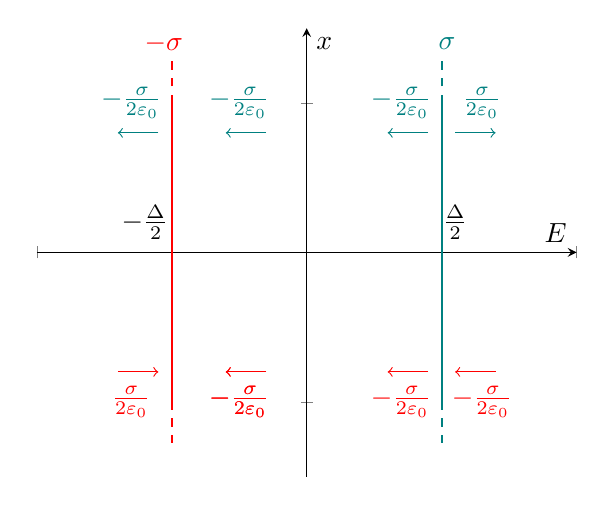
\begin{tikzpicture}
\begin{axis}[
%axis lines = left,
axis x line = center,
axis y line = middle,
xlabel = $E$,
ylabel = $x$,
ymax = 1.5,
ymin = -1.5,
xmax = 2,
xmin = -2,
xtick = {-2,-1,0,1,2},
xticklabels = {, , ,},
ytick = {-2,-1,0,1,2},
yticklabels = { , , , , }
]

\addplot [teal,thick] coordinates {(1,-1) (1,1)};
\addplot [teal,thick,dashed] coordinates {(1,1) (1,1.3)};
\addplot [teal,thick,dashed] coordinates {(1,-1) (1,-1.3)};

\addplot [red,thick] coordinates {(-1,-1) (-1,1)};
\addplot [red,thick,dashed] coordinates {(-1,-1) (-1,-1.3)};
\addplot [red,thick,dashed] coordinates {(-1,1) (-1,1.3)};

\addplot [->,teal] coordinates {(1.1,0.8) (1.4,0.8)};
\addplot [->,teal] coordinates {(0.9,0.8) (0.6,0.8)};
\node [teal] at (axis cs: 1.3,1) {$\frac{\sigma}{2\varepsilon_0}$};
\node [teal] at (axis cs: 0.7,1) {$-\frac{\sigma}{2\varepsilon_0}$};

\addplot [->,teal] coordinates {(-0.3,0.8) (-0.6,0.8)};
\node [teal] at (axis cs: -0.5,1) {$-\frac{\sigma}{2\varepsilon_0}$};

\addplot [->,teal] coordinates {(-1.1,0.8) (-1.4,0.8)};
\node [teal] at (axis cs: -1.3,1) {$-\frac{\sigma}{2\varepsilon_0}$};

\node[] at (axis cs: -1.2,0.2) {$-\frac{\Delta}{2}$};
\node[] at (axis cs: 1.1,0.2) {$\frac{\Delta}{2}$};
\node [teal] at (axis cs: 1.04,1.4) {$\sigma$};
\node [red] at (axis cs: -1.06,1.4) {$-\sigma$};

\addplot [->,red] coordinates {(-1.4,-0.8) (-1.1,-0.8)};
\node [red] at (axis cs: -1.3,-1) {$\frac{\sigma}{2\varepsilon_0}$};

\addplot [->,red] coordinates {(-0.3,-0.8) (-0.6,-0.8)};
\node [red] at (axis cs: -0.5,-1) {$-\frac{\sigma}{2\varepsilon_0}$};

\addplot [->,red] coordinates {(-0.3,-0.8) (-0.6,-0.8)};
\node [red] at (axis cs: -0.5,-1) {$-\frac{\sigma}{2\varepsilon_0}$};

\addplot [->,red] coordinates {(0.9,-0.8) (0.6,-0.8)};
\node [red] at (axis cs: 0.7,-1) {$-\frac{\sigma}{2\varepsilon_0}$};

\addplot [->,red] coordinates {(1.4,-0.8) (1.1,-0.8)};
\node [red] at (axis cs: 1.3,-1) {$-\frac{\sigma}{2\varepsilon_0}$};

\end{axis}
\end{tikzpicture}
\caption{Andamento del campo attraverso due lastre cariche}
\label{fig:lastre_indefinite}
\end{figure}

Siano due lastre poste a distanza $\Delta$ con carica $\sigma$ e $-\sigma$,
si avrà un campo pari a $\frac{\sigma}{2\varepsilon_0}$ a destra della
lastra $\sigma$ e $-\frac{\sigma}{2\varepsilon_0}$ nel lato sinistro della lastra.
Viceversa la lastra sinistra $-\sigma$ avrà verso opposto, applicando la sovrapposizione degli 
effetti si vede che il campo è nullo all'esterno dei due piani e pari a $-\sigma/\varepsilon_0$ 
nel mezzo.
$$
E_z = \begin{cases}
0, & |z| > \frac{\Delta}{2}\\
-\frac{\sigma}{\varepsilon_0}, & |z| \leq \frac{\Delta}{2}
\end{cases}
$$
Questa situazione è analoga a quella presente in un condensatore.

\section{Elettrostatica - Potenziale}
Si riportano le equazioni dell'elettrostatica
$$
\oiint_\Sigma \vec{E}\cdot\hat{n} dS = \frac{Q_{\Omega_\Sigma}}{\varepsilon_0}\ \ \forall\ \Sigma \text{ chiusa}
$$
$$
\oint_\Gamma \vec{E}\cdot\hat{t} dl =0\ \ \forall\ \Gamma \text{ chiusa}
$$
In forma locale diventano
$$
\nabla\cdot\vec{E} = \frac{\rho}{\varepsilon_0} \text{ in } \Omega \text{ punti regolari}
$$
L'equazione di Faraday-Neumann diventa:
$$
\nabla \times \vec{E} = 0 \text{ in } \Omega \text{ punti regolari}
$$
Le condizioni di raccordo si scrivono come:
$$
\begin{aligned}
\hat{n}\cdot (\vec{E}_2 - \vec{E}_1) &= \frac{\sigma}{\varepsilon_0} \text{ su } \partial\Omega\\
\hat{n}\times (\vec{E}_2 - \vec{E}_1) &= 0 \text{ su } \partial\Omega
\end{aligned}
$$

Se il dominio $\Omega$ è a connessione lineare semplice si ottiene l'equazione di \textit{Poisson}
$$
\nabla\times\vec{E} = 0 \Rightarrow \vec{E} = - \nabla V \text{ in } \Omega \Rightarrow \nabla^2V = -\frac{\rho}{\varepsilon_0} \text{ in } \Omega
$$
Sulla frontiera di $\Omega$: (condizione di raccordo per la funzione potenziale)
$$
\hat{n}\cdot (\vec{E}_2 - \vec{E}_1) = \hat{n}\cdot\left(-\nabla V_2 + \nabla V_1\right) =
\frac{\sigma}{\varepsilon_0} \Leftrightarrow
-\frac{\partial V_2}{\partial n} + \frac{\partial V_1}{\partial n} = \frac{\sigma}{\varepsilon_0}
$$
Continuità della componente tangente del campo elettrico:
$$
\hat{n}\times\left(\vec{E}_2-\vec{E}_1\right) = 0 \Rightarrow \hat{n}\times\left(-\nabla V_2 + \nabla V_1\right) = 0 \Rightarrow \hat{n}\times\left(-\nabla V_2 + \nabla V_1\right)\cdot\hat{m} = 0
$$
con $\hat{m}$ versore qualsiasi non parallelo ad $\hat{n}$, si prende ad esempio il versore $\hat{m}$
ortogonale alla linea chiusa rettangolare che interseca la superficie del dominio, 
il versore $\hat{t}$ sarà dunque dato dal prodotto vettoriale $\hat{t} = \hat{n}\times\hat{m}$ 
e risulterà tangente alla linea chiusa secondo il verso antiorario.
Sfruttando la proprietà circolare del prodotto misto:
$$
\begin{aligned}
\hat{t}\cdot\left(\nabla V_2 - \nabla V_1\right)  = 0 &\Rightarrow \frac{\partial V_2}{\partial \hat{t}} - \frac{\partial V_1}{\partial \hat{t}} = 0 \\
\frac{\partial}{\partial \hat{t}}(V_2-V_1)  = 0 &\Rightarrow V_2 = V_1
\text{ lungo la direzione }\hat{t}
\end{aligned}
$$
La continuità di $\hat{n}\times\vec{E}$ implica la continuità della funzione potenziale attraverso le superfici data l'arbitrarietà di $\hat{t}$.

\subsection{Funzioni armoniche}
Supponiamo che la carica $\rho$ sia nulla in $\Omega$, allora
$$
\nabla^2 V = 0 \text{ in } \Omega \text{ equazione di Laplace}
$$
le soluzioni dell'equazione di Laplace sono funzioni armoniche in $\Omega$.

\paragraph{Proprietà delle funzioni armoniche}
\subparagraph{Proprietà di unicità della soluzione}
Supponiamo di analizzare un problema di valori al contorno (BVP = \textit{Boundary Value Problem})

Problema di Dirichlet per l'equazione di Laplace:
$$
\begin{cases}
\nabla^2 V = 0 \text{ in } \Omega\\
\left.V\right|_{\partial\Omega} = h \text{ su } \partial\Omega
\end{cases}
$$
Ammette una e una sola soluzione.
L'unicità si dimostra con l'identità di Green:
$$
\nabla\cdot(f\nabla f) = f\nabla^2f + (\nabla f)^2
$$
Si integra utilizzando il teorema della divergenza:
$$
\begin{aligned}
\iiint_\Omega \nabla\cdot(V\nabla V) &= \cancel{\iiint_\Omega V\nabla^2 V dV} + \iiint_\Omega (\nabla V)^2 dV\\
\iint_{\partial\Omega} V \frac{\partial V}{\partial n}dS &= \iiint_\Omega (\nabla V)^2 dV
\end{aligned}
$$
Questo vale per una qualunque soluzione del problema.

Supponiamo $V_1$ e $V_2$ soluzioni. Def $\Delta V = V_1 - V_2$ 
$$
\begin{cases}
\nabla^2 (\Delta V) = 0 & \text{ in }\Omega \\
\left.\Delta V\right|_{\partial \Omega} = 0 \text{ su } \partial \Omega
\end{cases}
$$
Applicando la precedente identià di Green:
$$
\iint_{\partial \Omega} \Delta V \frac{\partial \Delta V}{\partial n} dS =
\iiint_\Omega \left[\nabla(\Delta V)\right]^2 dV = 0
$$
Perchè $\Delta V = 0$ sulla frontiera del dominio.
Il secondo termine può essere nullo se la funzione integranda è nulla in $\Omega$ ma se il dominio
è connesso:
$$
\nabla(\Delta V) = 0 \text{ in } \Omega \Rightarrow \Delta V = \text{cost in } \Omega \stackrel{\Delta V = 0 \text{ in }\partial\Omega}{\Rightarrow}
\Delta V = 0 \text{ in } \Omega \Rightarrow V_1 = V_2 \text{ in } \Omega
$$
L'unicità della soluzione continua a valere anche se $\Omega$ è illimitato assumendo che V sia 
normale all'infinito ($V \to 0 \text{ se } r \to \infty$).

\subparagraph{Principio del massimo delle funzioni armoniche}
Una funzione armonica in un dominio $\Omega$ assume valori estremi (i massimi e i minii) sulla
frontiera, se $V$ è costante su una superficie $\Sigma$, necessariamente deve essere costante
nella regione racchiusa $\Omega_\Sigma$ (se definita nella suddetta regione).

Se si riesce ad individuare una superficie sulla quale la funzione armonica è costante, nel caso
del potenziale si chiamano superfici equipotenziali, necessariamente all'interno della regione
racchiusa da questa superficie la funzione potenziale è costante.

\subparagraph{Problema di Neumann per l'equazione di Laplace}
Considerato sempre un dominio $\Omega$ ricerchiamo una funzione armonica in omega con derivata 
sulla frontiera assegnata di valore $g$
$$
\begin{cases}
\nabla^2 V = 0 \text{ in } \Omega\\
\left.\frac{\partial V}{\partial\hat{n}}\right|_{\partial \Omega} = g \text{ su } \partial \Omega
\end{cases}
$$
Si può dimostrare che le soluzioni del teorema di Neumann differiscono per una
costante additiva, invocando l'identità di Green:
$$
\begin{aligned}
\iiint_{\Omega} \left[\nabla(\Delta V)\right]^2 dV &= \iint_{\partial\Omega} \Delta V \frac{\partial\Delta V}{\partial \hat{n}} dS \stackrel{\partial\Delta V/\partial n = 0 }{=} 0\\
\nabla(\Delta V) &= 0 \text{ in } \Omega \Rightarrow \Delta V = \text{ cost in }\Omega 
\end{aligned}
$$

\subsection{Calcolo della funzione potenziale in condizioni di simmetria}
\paragraph{Carica puntiforme}
Sia posta una carica $Q$ nell'origine e $P_0$ un punto distante $r_0$ dall'origine e $P$ distante $r$ dall'origine.
Si suppone di estendere il raggio $r$ fino alla lunghezza di $r_0$ e di congiungere il punto $P'$
ottenuto con $p_0$ mediante una linea che giace sulla circonferenza di pari raggio.

$$
\vec{E}(P) = \frac{Q}{4\pi \varepsilon_0}\frac{1}{r^2} \vec{e}_r
$$
Integrando $\vec{E}$ lungo la curva $\gamma$ da $P$ a $P_0$
$$
\int_{P_\gamma P_0} \vec{E}\cdot \hat{t} dl = \int_{P_\gamma P_0} -\nabla V\cdot \hat{t} dl = 
\int_r^{r_0} \frac{Q}{4\pi\varepsilon_0}\frac{1}{r^2} \vec{e}_r\cdot \hat{t} dr + 
\cancel{\int_{P'}^{P_0} \vec{E}\cdot\hat{t} dl}
$$
ma $\vec{E}\cdot\hat{t} = 0$ perchè i due vettori sono ortogonali
$$
\int_r^{r_0} \frac{Q}{4\pi\varepsilon_0}\frac{1}{r^2}dr = \frac{Q}{4\pi\varepsilon_0}\left[-\frac{1}{r}\right]_r^{r_0} = \frac{Q}{4\pi\varepsilon_0}\left(\frac{1}{r} - \frac{1}{r_0}\right)
$$
$r_0$ e quindi $P_0$ funge da riferimento per la funzione potenziale, poichè $\vec{E} = -\nabla V$ 
tutte le funzioni potenziali che differiscono per una costante additiva costituiscono lo stesso
campo elettrico, in questo caso la costante è proprio $-\frac{Q}{4\pi\varepsilon_0}\frac{1}{r_0}$.
Si può quindi scegliere la costante di integrazione pari a $0$.

In genere quando le cariche sono al finito, conviene scegliere come funzione potenziale
$$
V(r) = \frac{Q}{4 \pi \varepsilon_0}\frac{1}{r}
$$

Tutte le scelte possibili sono valide, il potenziale è solo un artificio matematico
necessario a calcolare il campo che è la vera grandezza fisica.

Per ricavare il campo a partire dal potenziale è necessario calcolare il gradiente:
$$
\vec{E} = -\nabla V = \frac{Q}{4\pi\varepsilon_0}\frac{1}{r^2}\vec{e}_r
$$
pari proprio al campo della carica puntiforme.

Sia $Q$ una carica nell'origine e $P$ il raggio vettore che indica il punto in cui si vuole
calcolare il campo, le superfici ad $r$ costante hanno tutte lo stesso potenziale mentre
il campo è diretto in direzione radiale.

\paragraph{Potenziale generato da una distribuzione volumetrica $\rho$}
Sia $\Omega$ una regione carica con densità $\rho(p')$, con $p'$ interno ad $\Omega$ e raggio
vettore $\vec{r}_{p'}$, sia il punto in cui si vuole calcolare il campo $p$
allora la densità di carica elementare sarà $\rho(p')dV$, di conseguenza il potenziale in $p$
dovuto a $\rho(p')$ sarà:
$$
dV = \frac{\rho(p')dV}{4\pi\varepsilon_0}\frac{1}{|\vec{r}_p - \vec{r}_{p'}|} 
\stackrel{\text{PSE}}{\Rightarrow} \frac{1}{4\pi\varepsilon_0} \iiint_\Omega \frac{\rho(p')}{|\vec{r}_p - \vec{r}_{p'}|} dV = V(p) \text{ potenziale di Coulomb}
$$

$V(p)$ è continua $\forall P \in \mathbb{R}^3$ compresi i punti appartenenti ad $\Omega$, la 
singolarità è eventualmente integrabile dato che il volume infinitesimo $dV$ ha ordine 3 mentre la 
funzione integranda va come $\frac{1}{r}$.

\paragraph{Potenziale prodotto da distribuzione superficiale $\sigma$}
Sia $S$ la superficie con distribuzione superficiale $\sigma$ $p'$ un punto appartenente alla 
superficie e $p$ il punto in cui si calcola il potenziale.
$$
dV = \frac{\sigma(p')dS}{4\pi\varepsilon_0} \frac{1}{|\vec{r}_p - \vec{r}_{p'}|} 
\stackrel{\text{PSE}}{\Rightarrow}
\frac{1}{4\pi\varepsilon_0} \iint_S \frac{\sigma(p')}{|\vec{r}_p - \vec{r}_{p'}|} dS = V(p)
$$
Anche questa funzione è continua $\forall\ p \in \mathbb{R}^3$

\paragraph{Distribuzione lineare con densità $\lambda(p')$}
con $p'\in\gamma$ 
$$
dV = \frac{\lambda(p')dl}{4\pi\varepsilon_0}\frac{1}{|\vec{r}_p-\vec{r}_{p'}|} 
\stackrel{\text{PSE}}{\Rightarrow} V(p) = \frac{1}{4\pi\varepsilon_0} 
\int_\gamma \frac{\lambda(p')}{|\vec{r}_p-\vec{r}_{p'}|}dl
$$
Questa funzione è continua $\forall p \notin \gamma $ dato che diverge logaritmicamente su $\gamma$.

\subsection{Operatori differenziali in coordinate curvilinee}
Sia $\Delta\Omega$ un volumetto elementare in $P$ in cui si pone un sistema di coordinate
locali $l_1,l_2,l_3$, il volumetto ha dimensioni $dl_1,\ dl_2,\ dl_3$.
Siano $(u_1,u_2,u_3)$ un sistema di coordinate curvilinee ortogonali, 
gli spostamenti elementari saranno:
\begin{align*}
dl_1 &= h_1du_1\\
dl_2 &= h_2du_2\\
dl_3 &= h_3du_3
\end{align*}
Con $h_1,h_2,h_3$ i fattori metrici che dipendono dal punto.

Le superfici coordinate elementari:
\begin{align*}
dS_1 &= dl_2dl_3 = h_2h_3du_2du_3\\
dS_2 &= dl_3dl_1 = h_3h_1du_3du_1\\
dS_3 &= dl_1dl_2 = h_1h_2du_1du_2
\end{align*}

Volume elementare:
$$
dV = dl_1dl_2dl_3 = h_1h_2h_3du_1du_2du_3
$$

\paragraph{Operatore Divergenza in coordinate curvilinee}
Operando la definizione intrinseca la divergenza è il rapporto fra il flusso attraverso la 
superficie del volume elementare e il volume elementare stesso:

$$
\vec{v}(p) \in \mathbb{C}^1(\Omega) :
$$
$$
\nabla\cdot\vec{v} = \frac{\iint_{\partial\Delta\Omega}\vec{v}\cdot\hat{n}dS}{\text{Vol}(\Delta \Omega)}
= \frac{1}{dV} \left[\begin{aligned}
&\vec{v}\left(u_1+\frac{du_1}{2},u_2,u_3\right)\cdot\vec{e}_1\cdot
dS_1\left(u_1+\frac{du_1}{2},u_2,u_3\right) - \\
&\vec{v}\left(u_1-\frac{du_1}{2},u_2,u_3\right)\cdot\vec{e}_1\cdot
dS_1\left(u_1-\frac{du_1}{2},u_2,u_3\right) + \\
&\vec{v}\left(u_1,u_2+\frac{du_2}{2},u_3\right)\cdot\vec{e}_2\cdot
dS_2\left(u_1,u_2+\frac{du_2}{2},u_3\right)  - \\
&\vec{v} \left(u_1,u_2-\frac{du_2}{2},u_3\right)\cdot\vec{e}_2\cdot
dS_2\left(u_1,u_2-\frac{du_2}{2},u_3\right) + \\
&\vec{v} \left(u_1,u_2,u_3+\frac{du_3}{2}\right)\cdot\vec{e}_3\cdot
dS_3\left(u_1,u_2,u_3+\frac{du_3}{2}\right) - \\
&\vec{v} \left(u_1,u_2,u_3-\frac{du_3}{2}\right)\cdot\vec{e}_3\cdot
dS_3\left(u_1,u_2,u_3-\frac{du_3}{2}\right)
\end{aligned} \right]
$$
Si considerano i primi due termini ricordando che $dV = h_1h_2h_3du_1du_2du_3$
$$
\begin{aligned}
&\nabla\cdot\vec{v} = \frac{1}{h_1h_2h_3} \cdot \\
&\left[\frac{v_1(u_1+\frac{du_1}{2},u_2,u_3)dS_1(u_1+\frac{du_1}{2},u_2,u_3) - v_1(u_1-\frac{du_1}{2},u_2,u_3)dS_1(u_1-\frac{du_1}{2},u_2,u_3)+...}{du_1du_2du_3}\right]
\end{aligned}
$$
ma $dS_1 = [h_2h_3](u_1+\frac{du_1}{2},u_2,u_3)du_2du_3$
quindi semplificando i termini $du_2du_3$ si ottiene:
\begin{equation}
\nabla\cdot\vec{v} = \frac{1}{h_1h_2h_3}\left[\frac{\partial}{\partial u_1}(v_1h_2h_3) +
\frac{\partial}{\partial u_2}(v_2h_1h_3) + \frac{\partial}{\partial u_3}(v_3h_1h_2)\right]
\label{eq:divergenza_curvilinea}
\end{equation}
Quella appena ricavata è l'espressione dell'operatore divergenza per un qualsiasi 
sistema di coordinate curvilineo ortogonale.

\paragraph{Laplaciano in coordinate curvilinee}
Si ricorda la definizione di gradiente di un campo scalare:
$$
\nabla f = \frac{1}{h_1} \frac{\partial f}{\partial u_1} \vec{e}_1 +
\frac{1}{h_2} \frac{\partial f}{\partial u_2} \vec{e}_2 + 
\frac{1}{h_3} \frac{\partial f}{\partial u_3} \vec{e}_3
$$
Utilizzando la \ref{eq:divergenza_curvilinea} appena ricavata si ottiene il laplaciano $\nabla^2 f = \nabla\cdot(\nabla f) $

$$
\nabla^2 f = \frac{1}{h_1h_2h_3} \left[ \frac{\partial}{\partial u_1}
\left(\frac{h_2h_3}{h_1}\frac{\partial f}{\partial u_1}\right) + 
\frac{\partial}{\partial u_2}
\left(\frac{h_1h_3}{h_2}\frac{\partial f}{\partial u_2}\right) + 
\frac{\partial}{\partial u_3}
\left(\frac{h_1h_2}{h_3}\frac{\partial f}{\partial u_3}\right)\right]
$$
\subparagraph{Coordinate sferiche}
$$
\nabla^2 f = \frac{1}{r^2\sin\vartheta} \left[\frac{\partial}{\partial r}\left(r^2\sin\vartheta\frac{\partial f}{\partial r}\right)+
\frac{\partial}{\partial \vartheta}\left( \frac{\cancel{r}\sin\vartheta}{\cancel{r}}\frac{\partial f}{\partial \vartheta}\right) +
\frac{\partial}{\partial \varphi}\left( \frac{\cancel{r}}{\cancel{r}\sin\vartheta}\frac{\partial f}{\partial \varphi}\right) \right] =
$$
$$
\frac{1}{r^2}\frac{\partial}{\partial r} \left(r^2 \frac{\partial f}{\partial r} \right) 
+ \frac{1}{r^2 \sin\vartheta}\frac{\partial}{\partial \vartheta} \left(\sin \vartheta \frac{\partial f}{\partial \vartheta}\right) +
\frac{1}{r^2\sin^2\vartheta} \frac{\partial^2 f}{\partial \varphi^2}
$$
Si vede dunque che $h_1=1,\ h_2=r,\ h_3 = r\sin\vartheta$
\subparagraph{Coordiante cilindriche}
$$
\begin{aligned}
\nabla^2 f &= \frac{1}{r} \left[\frac{\partial}{\partial r}\left(r\frac{\partial f}{\partial r} \right) + \frac{\partial}{\partial \phi}\left(\frac{1}{r}\frac{\partial f }{\partial \phi} \right) + \frac{\partial}{\partial z} \left(r \frac{\partial f}{\partial z}\right) \right] = \\
\nabla^2 f &= \frac{1}{r}\frac{\partial}{\partial r} \left(r\frac{\partial f }{\partial r}\right) + \frac{1}{r^2}\frac{\partial^2 f}{\partial \phi^2} + \frac{\partial^2 f}{\partial z^2}
\end{aligned}
$$

\paragraph{Distribuzione di carica superficiale con simmetria sferica}
Si consideri un guscio sferico di raggio $R$, si definisce 
$\sigma(R,\vartheta,\varphi) = \sigma_0$, determinare potenziale e campo elettrico in
tutto lo spazio.

Formulazione del problema: $V(P) = V(r)$ a causa della simmetria, il problema
è monodimensionale, la funzione potenziale dipende da una sola variabile.
Si definisce regione $(1)$ quella interna alla sfera e regione $(2)$ quella esterna.
$$\begin{cases}
\nabla^2 V_1 = 0, & \text{ in } 0\leq r\leq R \\
\nabla^2 V_2 = 0, & \text{ in } r > R \\
V_1(R) = V_2(R), &\text{ continuità del potenziale} \\
-\frac{\partial V_2}{\partial n} + \frac{\partial V_1}{\partial n} = \frac{\sigma_0}{\varepsilon_0}, & \text{ su } \Sigma : r=R \\
\lim_{r\to\infty} V_2(r) = 0, & V_2 \text{ normale all'}\infty
\end{cases}
$$
Queste ipotesi garantiscono che la soluzione sia unica.
Sriscrive l'espressione del Laplaciano in coordinate sferiche, prendendo solo la parte
che dipende da $r$ a causa della simmetria del problema.
$$
\frac{1}{r^2}\frac{\partial}{\partial r} \left(r^2 \frac{\partial V}{\partial r}\right) = 0 \stackrel{r\neq 0}{\Rightarrow} \frac{\partial}{\partial r} \left(r^2 \frac{\partial V}{\partial r}\right) = 0 \Rightarrow r^2 \frac{\partial V}{\partial r} = A \Rightarrow
\frac{\partial V}{\partial r} = \frac{A}{r^2} \Rightarrow V(r) = -\frac{A}{r} + B
$$
Utilizzando le condizioni per la continuità del potenziale e la discontinuità della
sua derivata normale vanno determinate le costanti relative ai due domini.
$$
V_1(r) = -\frac{A}{r} + B \ \ \ V_2(r) = -\frac{C}{r} + D
$$
con $A,B,C,D$ costanti di integrazione da determinare utilizzando le condizioni
di raccordo e al contorno.
